\sffamily
Here you can see how to include an image in your document.

\begin{sidewaysfigure}
\centering
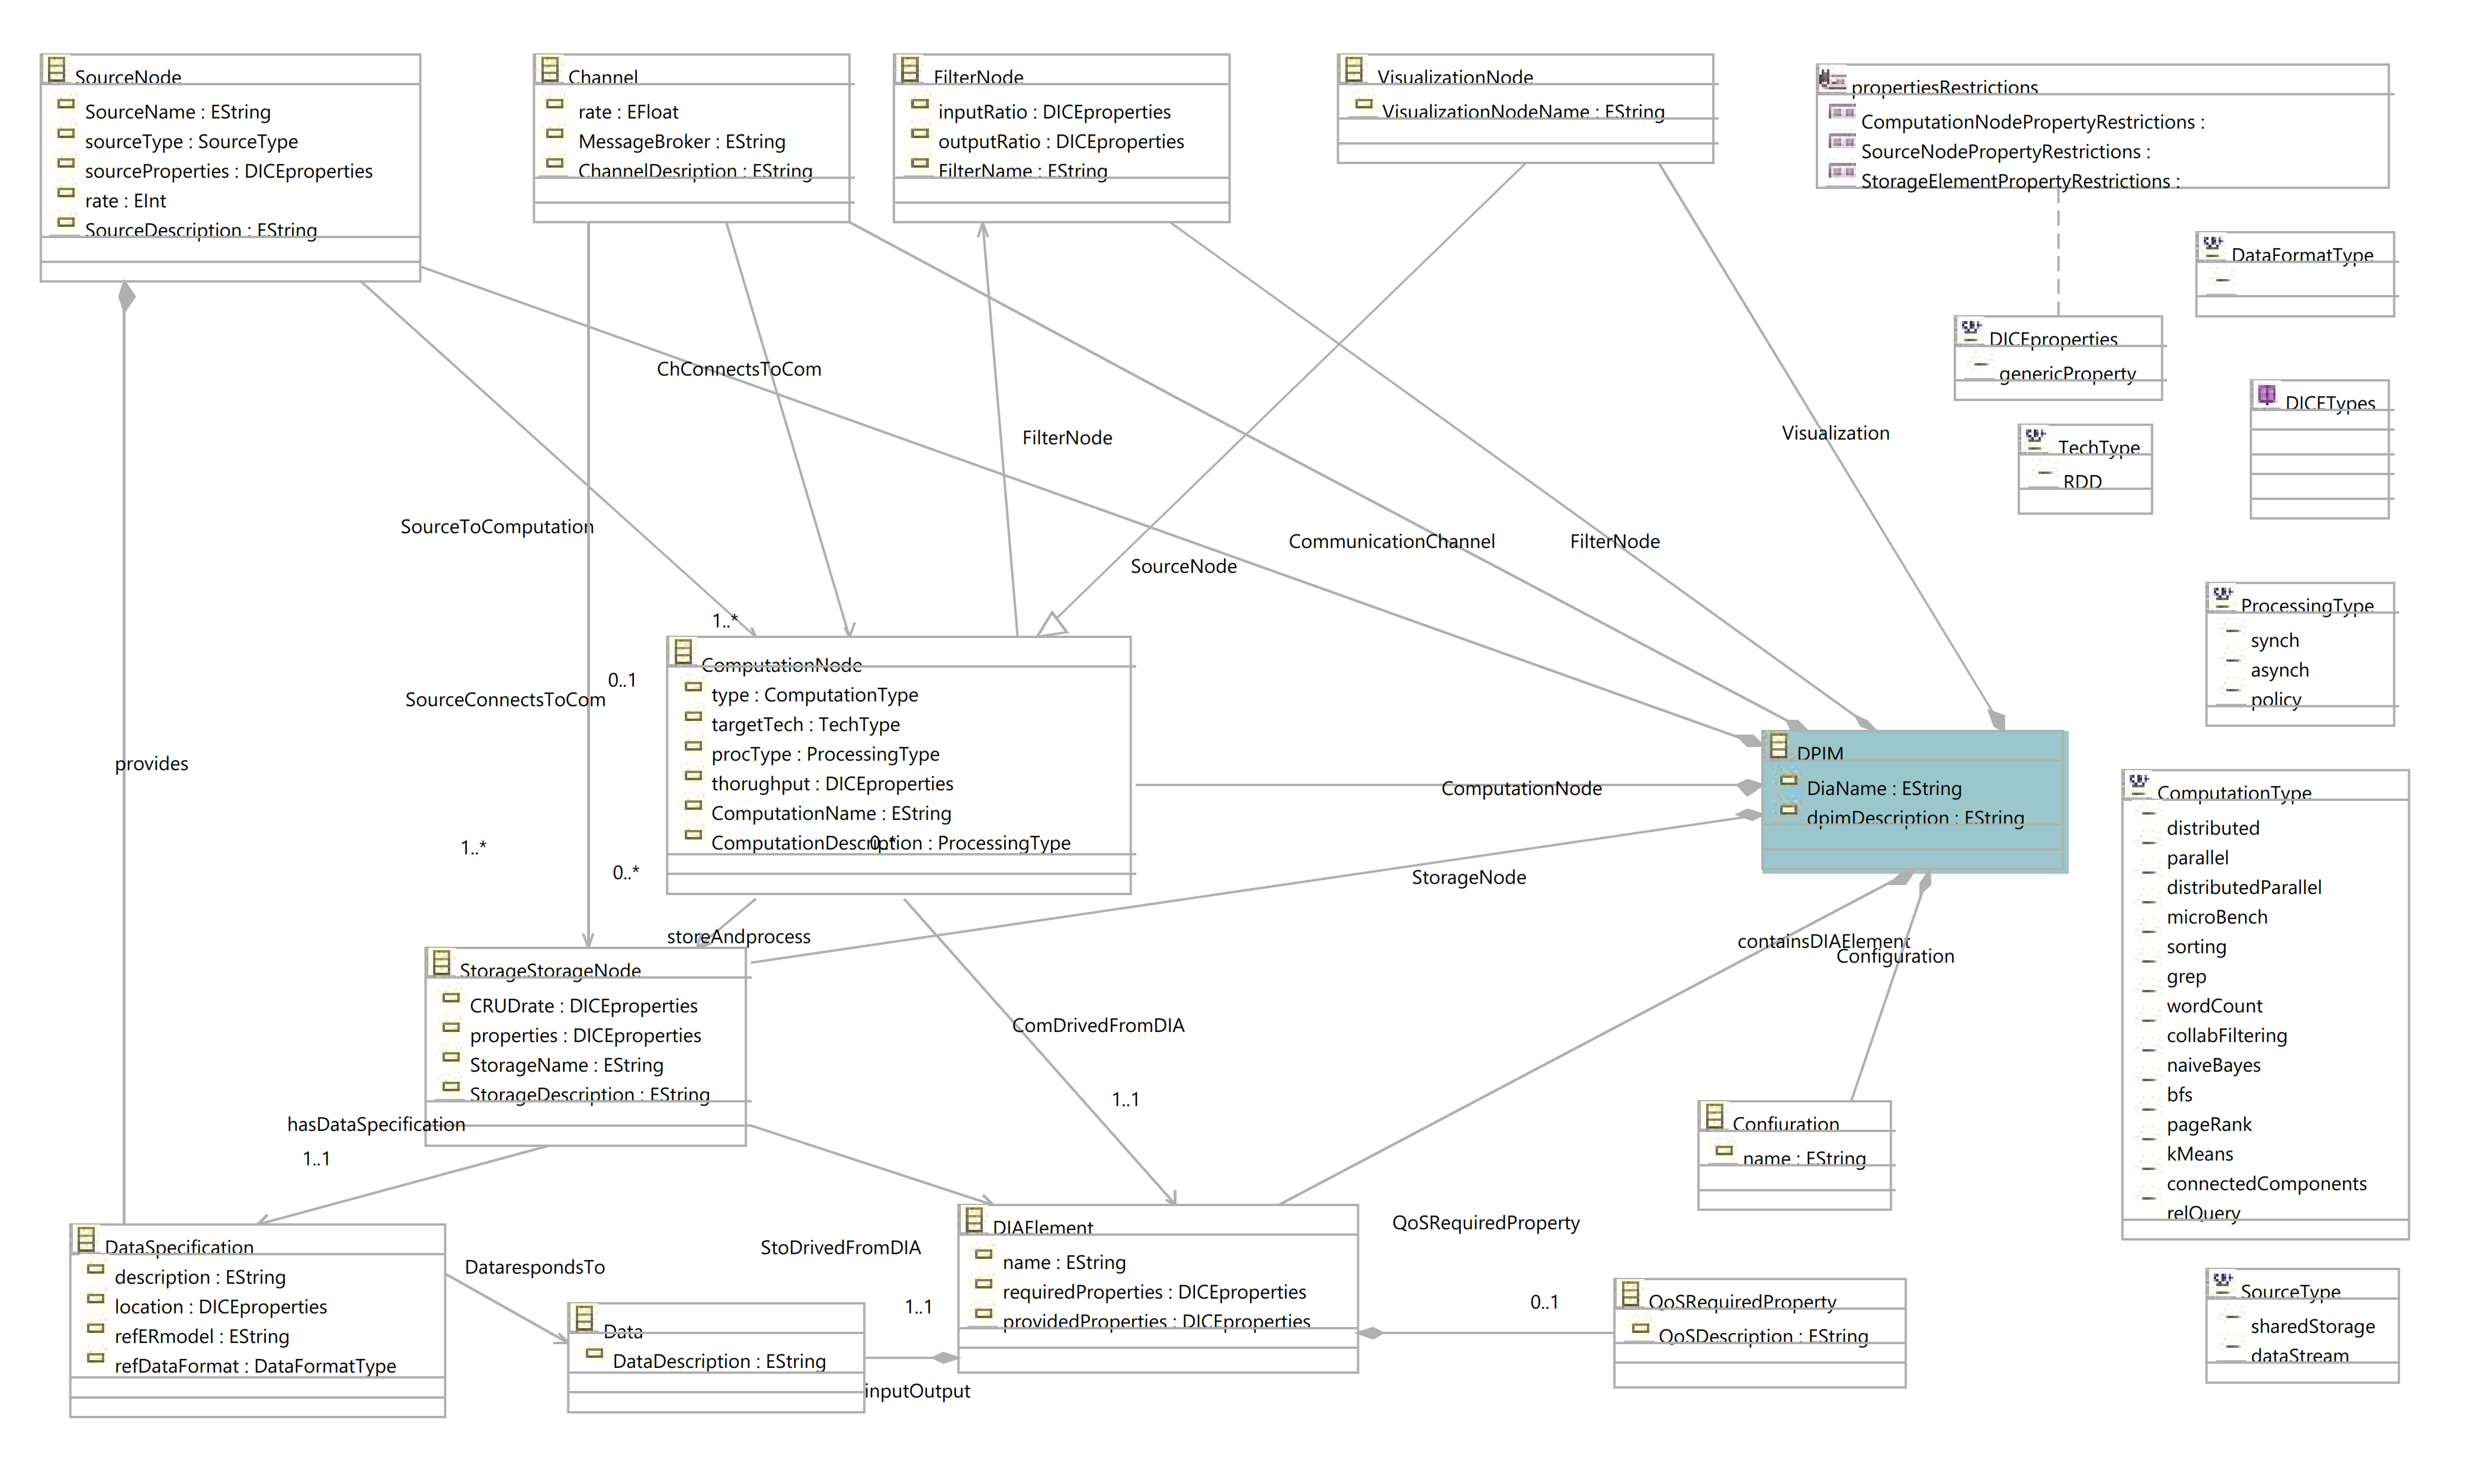
\includegraphics[width=\textwidth]{Images/11.png}
\caption{\label{fig:metamodel}DICE DPIM metamodel.}
\end{sidewaysfigure}

\begin{figure}
\centering
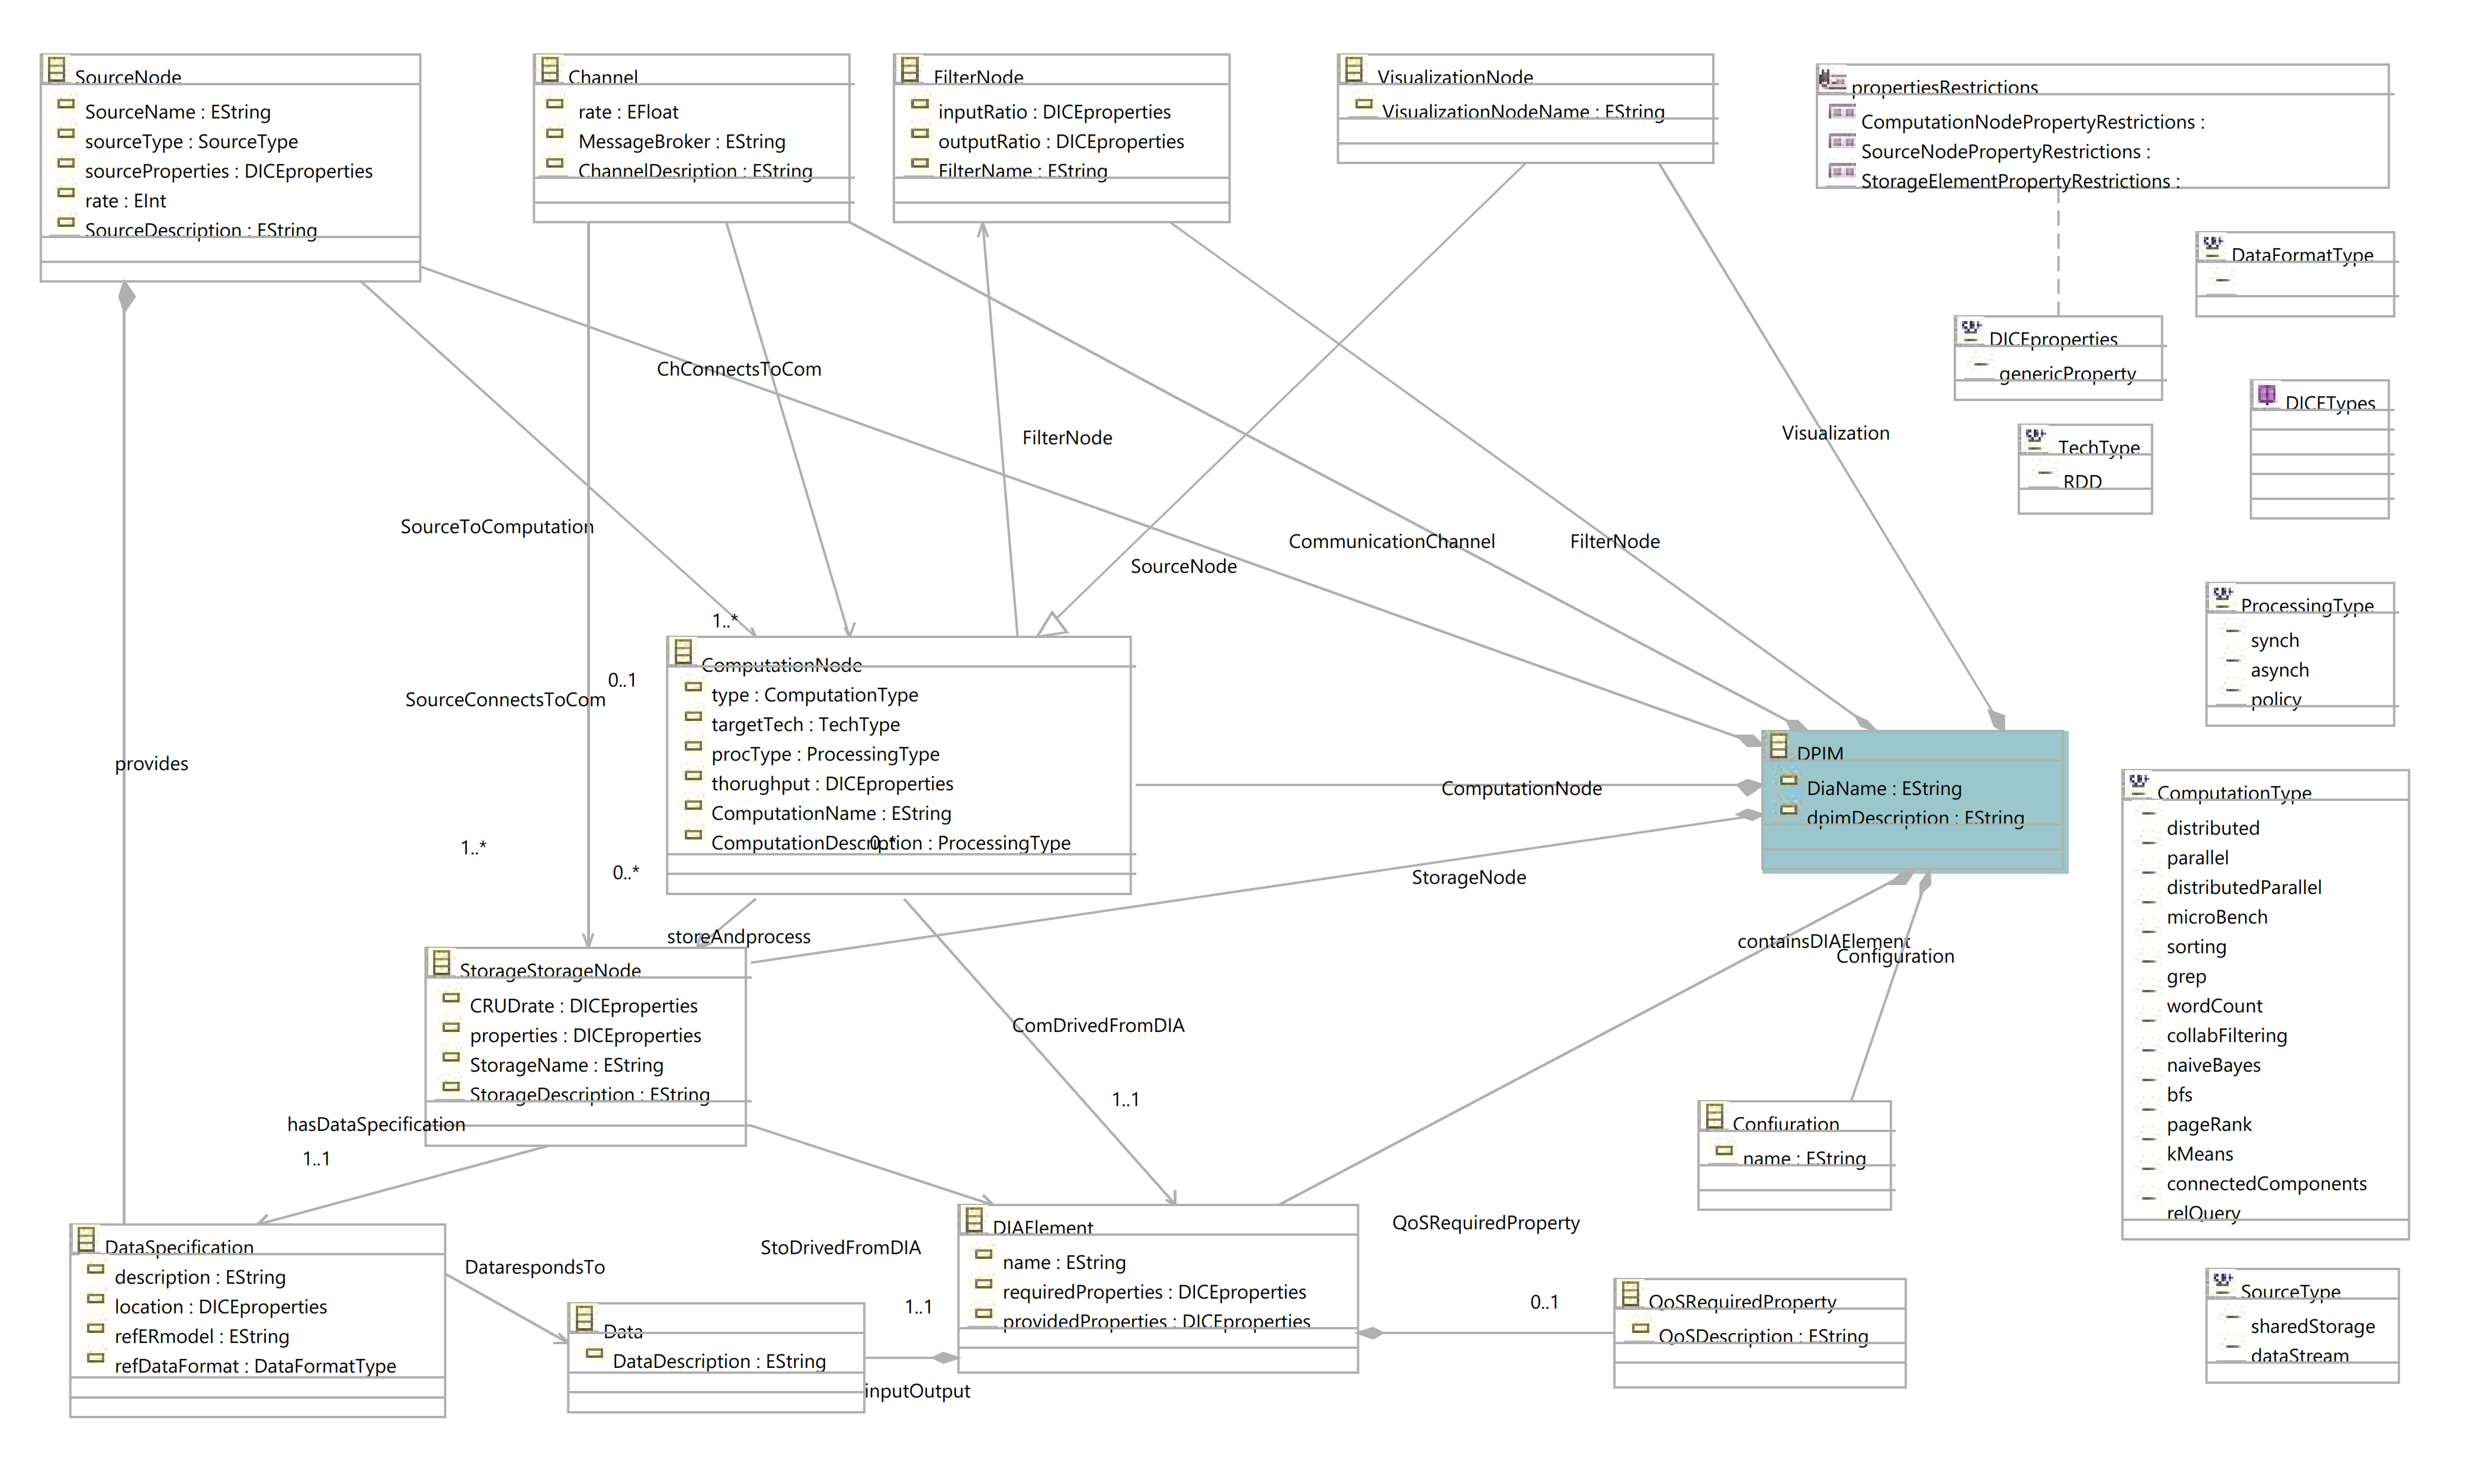
\includegraphics[width=\textwidth]{Images/11.png}
\caption{\label{fig:metamodel2}DICE DPIM metamodel in portrait form.}
\end{figure}

Here is the command to refer to another element (section, figure, table, ...) in the document: \emph{As discussed in Section~\ref{sect:overview} and as shown in Figure~\ref{fig:metamodel}, ...}. Here is how to introduce a bibliographic citation~\cite{DAM}. Bibliographic references should be included in a \texttt{.bib} file. 

Table generation is a bit complicated in Latex. You will soon become proficient, but to start you can rely on tools or external services. See for instance this \href{https://www.tablesgenerator.com}{https://www.tablesgenerator.com}. \\

\subsection{\sffamily Product Perspective}
\subsubsection{\sffamily Scenarios}
\paragraph{Scenario 1}

Single user of the CLup platform, Bob, decides it's time to go shopping.
Bob lives in Milan and this means he's currently in reach of 5 different supermarkets belonging to the CLup network. \newline
Bob then opens the app, checks the status of the current queue and notices the nearest supermarket has free room, 13 entrances left out of 55 total. It's fine for Bob, he starts walking towards it. \newline
As soon as he approaches the supermarket (Bob's on foot), he checks the app and start the check-in procedure. It's not rush hours and 8 entrance are still left, so everything goes ok and Bob gets a QR ticket. He approaches the entrance, has is code scanned by an automatic turnstile and gets inside the supermarket.\newline
In 36' time, Bob completes his shopping. He proceeds towards the exit, where another turnstile scans his QR code once again to confirm exit. He's now free to get home.

\subsection{Product Functions}

\subsection{User Characteristics}

\subsection{Assumptions, Dependencies and Constraints}
\subsubsection{Domain Assumptions}
Follows a list of assumptions made about the domain CLup focuses on.\newline\newline
\begin{tabular}{l|l}
	D1 & Entrance checking is possible and guaranteed by the Staff\\
	D2 & Exit checking is possible and guaranteed by the Staff\\
	D3 & One customer per authorization given is allowed in by the Staff\\
	
\end{tabular}
